\chapter{Implementation}
\label{chap:imp}
\lhead{\emph{Project Implementation}}
This chapter details the development process of the Docker Linter Project, transitioning from the planned approach outlined in Chapter 4 to the final implemented solution. It documents the practical challenges encountered during the implementation phase (January - April), categorizes their severity, and analyzes their impact on the project's design, schedule, and outcomes. Furthermore, it provides an "as-built" specification by comparing the original plan (architecture, use cases, risks, methodology, schedule, evaluation, prototype) with the final developed project, justifying deviations based on the encountered difficulties.
\begin{itemize}
    \item \textbf{Easy:} The Challenge was easily resolved
    \item \textbf{Medium:} A significant challenge that required thought, research and problem solving to resolve
    \item \textbf{Hard:} Otherwise known as a blocker, a challenge that was too complex to resolve
and caused changes to the project’s functional and/or non-functional requirements
\end{itemize}
\section{Difficulties Encountered}
\label{sec:difficulties}
The development phase involved several technical and logistical challenges. These are categorized below based on their complexity and impact on the project's progression.

% --- Difficulty 1: LLM for Regex Generation ---
\subsection{Automating Rule Generation (English to Regex) using LLMs}
\label{subsec:llm_regex_difficulty} % Added label for potential cross-referencing
\begin{itemize}
    \item \textbf{Classification:} Hard
    \item \textbf{Description:} A significant challenge arose when attempting to automate the conversion of Docker best practices, often described in natural English, into precise regular expressions (Regex) suitable for the linter's rule engine. The goal was to leverage Large Language Models (LLMs) like gpt-4o to parse best practice descriptions (e.g., from docker official documentation ) and automatically generate corresponding Regex patterns. Despite experimenting with multiple LLMs and refining prompts to provide clear instructions and examples, the results were consistently unsatisfactory. The generated Regex patterns suffered from:
        \begin{itemize}
            \item \textbf{Inaccuracy:} Patterns often failed to correctly capture the understanding of the best practice, leading to potential false positives or false negatives during linting.
            \item \textbf{Inconsistency:} Even with the same input, the models produced varying outputs, making it impossible to generate reliable rules.
            \item \textbf{Over-simplification or Over-complexity:} Patterns were sometimes too general, matching unintended lines, or overly complex and inefficient.
        \end{itemize}
    \item \textbf{Impact on Original Project Design:}
        \begin{enumerate}
            \item \textbf{Architecture:} This directly impacted the planned mechanism for rule creation and updates. The failure of LLM automation necessitated a fallback to manual or semi-automated methods, affecting the architecture of the rule management component (potentially requiring more robust manual entry/validation interfaces or processes than initially envisioned if automation was heavily relied upon). It also impacted the envisioned workflow for updating rules based on newly scraped best practices.
            \item \textbf{Risk:} This represented an unforeseen technical risk not explicitly detailed in the initial assessment (Chapter 4, Section 4.2). While "Rule Conflicts" (Risk 6) and "Outdated Scraped Rules" (Risk 5) were identified, the difficulty of translating potentially valid scraped information into usable rules was underestimated. The failure introduced a risk of lower rule coverage or accuracy if manual generation couldn't keep pace or achieve the desired precision.
            \item \textbf{Methodology:} The Agile approach allowed for adapting to this challenge. Time initially allocated to LLM experimentation and integration within sprints had to be reallocated to manual rule creation and testing, demonstrating the methodology's flexibility.
            \item \textbf{Schedule:} Significant time was invested in exploring the LLM approach during the initial implementation phase (January-February). When this proved unsuccessful, it caused delays in populating the rule database,impacting subsequent tasks like comprehensive testing and IDE integration refinement which relied on a robust rule set. The schedule needed adjustment to accommodate the increased effort for manual rule generation.
            \item \textbf{Evaluation Plan:} The failure to automate rule generation meant relying on manual creation. This could impact the evaluation of smell detection (precision/recall) if the resulting rule set was less comprehensive than initially planned.
        \end{enumerate}
\item \textbf{Management Strategy:} The approach of using LLMs to automatically generate Regex rules from English descriptions proved unreliable, producing inaccurate and inconsistent patterns. Consequently, this automation attempt was abandoned. The strategy shifted entirely to manual Regex rule creation, which involved:
    \begin{itemize}
        \item Analyzing best practice descriptions from reliable sources (like Docker documentation).
        \item Manually writing and testing Regex patterns against sample Dockerfile lines making the Database redundant. 
        \item Storing these validated rules in a structured format (e.g., JSON/YAML in \texttt{Rules/}) with necessary metadata (severity, description, suggestion), drawing from structures like \texttt{Rules.json}.
    \end{itemize}
    These carefully crafted manual rules provided a reliable foundation for the linter's analysis engine (including any AI-driven components that used these rules), ensuring accuracy. However, this came at the cost of slower development and potentially fewer rules than planned with automation.
\end{itemize}

% --- Difficulty 2: Web Scraper Reliability --- (Based on Risk 10)
\subsection{Web Scraper Reliability and Maintenance}
\label{subsec:scraper_difficulty}
\begin{itemize}
    \item \textbf{Classification:} Medium
    \item \textbf{Description:} The web scraper (\texttt{webscraper.py}), originally designed to fetch Docker best practices from online sources to populate a dynamic rule database (as planned in Chapter 4, Section 4.1.2), faced intermittent failures. Websites frequently change their structure (HTML layout, CSS selectors), breaking the parsing logic. Ensuring the scraper consistently fetched information required ongoing monitoring and adjustments. This aligns with the anticipated “Web scraper failure” risk (Risk 10).  
    \newline\textit{Note: Even though rule generation is now manual, the GPT-4o analysis engine still loads the scraper’s JSON output at runtime to stay informed of any newly scraped best practices.}

    \item \textbf{Impact on Original Project Design:}
        \begin{enumerate}
            \item \textbf{Architecture:} The failure of LLM-based rule generation (Section \ref{subsec:llm_regex_difficulty}) reduced the scraper’s role in directly feeding the linter’s active rule set. It now primarily serves as a discovery tool—its JSON output is consumed by GPT-4o for AI-driven analysis rather than auto-populating the database.
            \item \textbf{Risk:} Realized the high‐frequency “Web scraper failure” risk (Risk 10). Its reduced direct impact on rules did not eliminate the maintenance effort.
            \item \textbf{Methodology:} Sprints allocated time for scraper upkeep, though at lower priority given its secondary role.
            \item \textbf{Schedule:} Introduced minor, unpredictable delays for scraping fixes, with less effect on core linting development than originally anticipated.
            \item \textbf{Evaluation Plan:} Since dynamic rule updates via scraping are no longer automatic, evaluation of “Outdated Scraped Rules” shifted focus to manual review of discovered practices.
        \end{enumerate}

    \item \textbf{Management Strategy:} Even with its reduced role, we kept the scraper reliable as a discovery source and AI input:
        \begin{itemize}
            \item \textbf{Robust Error Handling:} Wrapped network calls and HTML parsing in \texttt{try-except} to catch connection or DOM‐change errors, preventing crashes.
            \item \textbf{Detailed Logging:} Used Python’s \texttt{logging} to record URLs, timestamps, success/failure status, and exceptions for quick diagnosis.
            \item \textbf{Simplified Validation:} Periodically ran the scraper against key sources to confirm basic functionality and data extraction.
            \item \textbf{Source Prioritization:} Focused on the most stable, authoritative sites (e.g., Docker docs) rather than broad diversification.
            \item \textbf{AI Integration:} Ensured GPT-4o reads the scraper’s JSON each run to refresh its knowledge of best practices—keeping AI analysis aligned with scraped sources even though rule enforcement is manual.
            \item \textbf{Reactive Maintenance:} Treated breakages as bugs, fixing selectors or parsing logic as part of routine sprint backlog grooming.
        \end{itemize}
\end{itemize}

% --- Difficulty 3: Dockerfile Optimization & Linter Application --- (Based on explanation.txt)
\subsection{Implementing Dockerfile Optimizations}
\label{subsec:optimization_difficulty}
\begin{itemize}
    \item \textbf{Classification:} Medium
    \item \textbf{Description:} Applying linter recommendations (multi-stage builds, non-root users, combining \texttt{RUN} steps, using \texttt{COPY} instead of \texttt{ADD}, pinning versions) to our own Dockerfile required careful testing to avoid build or runtime breakages.
    \item \textbf{Impact on Original Project Design:}
        \begin{enumerate}
            \item \textbf{Architecture:} Produced a more complex, multi-stage Dockerfile, improving deployment structure.
            \item \textbf{Risk:} Raised security and efficiency but occasionally triggered new build failures.
            \item \textbf{Methodology:} Used Agile's iterative cycles to implement and verify each change.
            \item \textbf{Schedule:} Allocated extra time for rebuilding and debugging after each optimization.
            \item \textbf{Evaluation Plan:} Showed image size reductions and faster builds, satisfying the "Optimising Performance" goal.
        \end{enumerate}
    \item \textbf{Management Strategy:} The project's own Dockerfile optimizations were applied and tested in a single workflow rather than step-by-step rebuilds:
        \begin{itemize}
            \item \textbf{AI-Driven Rewrite:} Generated a complete optimized Dockerfile via GPT-4o, incorporating linter findings and best practices.
            \item \textbf{Post-Processing:} Cleaned the AI output (e.g., removed incompatible version pins) to ensure compatibility with the chosen base image.
            \item \textbf{Single Build Verification:} Built the optimized image once to collect size and layer metrics.
            \item \textbf{Version Control:} Committed the final, verified Dockerfile with clear messages and used Git's rollback on any post-merge issues.
            \item \textbf{Documentation:} Added inline comments in the Dockerfile and descriptive commit notes explaining each major change and its benefit.
        \end{itemize}
\end{itemize}

% --- Difficulty 4: Integration Complexity (VS Code / Jenkins) ---
\subsection{Integration Complexity (VS Code / Jenkins)}
\label{subsec:integration_difficulty}
\begin{itemize}
  \item \textbf{Classification:} Medium
  \item \textbf{Description:} Integrating the linter with VS Code (\texttt{VS-Extension}) required understanding the VS Code API for diagnostics and commands. Similarly, setting up Jenkins pipelines (\texttt{jenkins}) to execute the linter (e.g.\ \texttt{lint\_cli.py}) involved configuring build steps, handling outputs, and managing execution environments. Specific API calls and pipeline syntax often needed troubleshooting and experimentation.
  \item \textbf{Impact on Original Project Design:} Primarily affected the schedule, requiring dedicated time for understanding external tool APIs and configurations. This directly tests the planned mitigation for Risk 1 (CI/CD integration testing).
  \item \textbf{Management Strategy:} Addressed external-tool complexities through focused research and iterative testing:
    \begin{itemize}
      \item \textbf{Targeted Documentation Review:} Consulted VS Code’s \texttt{DiagnosticCollection} and \texttt{commands} API docs, and Jenkins Pipeline syntax for \texttt{sh} steps, exit-code handling, and report plugins (e.g.\ Warnings NG).
      \item \textbf{Example-Driven Development:} Adapted community examples (Stack Overflow, official tutorials) to bootstrap extension and pipeline scripts.
      \item \textbf{Incremental Testing and Debugging:}
        \begin{itemize}
          \item \textbf{VS Code:} Verified the extension loads; tested lint on save/open; parsed JSON output from \texttt{lint\_cli.py} into diagnostics; added custom commands (e.g.\ ignore rule).
          \item \textbf{Jenkins:} 
            \begin{enumerate}
              \item Checkout code.
              \item Execute \texttt{sh 'python lint\_cli.py --format json || exit 1'} to fail on non-zero exit.
              \item Verify output in console logs.
              \item Put output into Jenkins artifacts ( like .csv files)
            \end{enumerate}
        \end{itemize}
    \end{itemize}
\end{itemize}
% --- Difficulty 5: Lack of Benchmark Datasets ---
\subsection{Lack of Public Benchmark Datasets for Evaluation}
\label{subsec:benchmark_difficulty}
\begin{itemize}
    \item \textbf{Classification:} Medium
    \item \textbf{Description:} A significant hurdle was encountered during the evaluation phase (Chapter 6) when attempting to find publicly available, standardized datasets of Dockerfiles with known, labeled vulnerabilities or "smells" (anti-patterns). While general code vulnerability datasets exist, datasets specifically curated for Dockerfile best practices and common security flaws targeted by this linter were scarce or non-existent. Existing Dockerfile collections often lacked ground-truth annotations regarding adherence to specific best practices (like those enforced by the linter's rules), making objective measurement of the linter's precision and recall difficult using external benchmarks.
    \item \textbf{Impact on Original Project Design:}
        \begin{enumerate}
            \item \textbf{Evaluation Plan:} This directly impacted the planned methodology for evaluating the linter's effectiveness (precision/recall metrics). The inability to use established benchmarks necessitated a pivot to creating a custom benchmark dataset, requiring additional time and effort not initially budgeted within the evaluation phase. It also meant the evaluation results would be based on this custom benchmark, potentially limiting direct comparability with other tools evaluated on different (hypothetical) datasets.
            \item \textbf{Risk:} Introduced the risk that the custom-created benchmark might not be fully representative of real-world Dockerfiles or could unintentionally favour the linter's specific rule set, potentially biasing the evaluation results.
            \item \textbf{Schedule:} Substantial time had to be allocated within the evaluation period (or potentially extending it) to curate, analyze, and label Dockerfiles for the custom benchmark.
        \end{enumerate}
    \item \textbf{Management Strategy:}
        \begin{itemize}
            \item \textbf{Custom Benchmark Creation:} Since no suitable public dataset was found, a custom benchmark dataset was manually created. This involved:
                \begin{itemize}
                    \item Collecting a diverse set of Dockerfiles from various sources (e.g., GitHub repositories, public examples, potentially anonymized internal projects) to ensure variety in complexity, base images, and application types.
                    \item Manually analyzing each Dockerfile against the linter's defined rule set (\texttt{Rules/}).
                    \item Carefully labeling each Dockerfile (or specific lines within them) with the ground truth – identifying which rules should be triggered (true positives) and which parts were compliant (true negatives).
                    \item Documenting the benchmark creation process and the criteria used for labeling to ensure transparency and potential reproducibility.
                \end{itemize}
            \item \textbf{Targeted Evaluation:} The evaluation metrics (precision, recall, F1-score) were then calculated based on the linter's performance against this custom-built, manually-labeled dataset.
            \item \textbf{Acknowledging Limitations:} The evaluation results explicitly noted that they were based on a custom benchmark due to the lack of public alternatives, acknowledging the potential limitations this entails.
        \end{itemize}
\end{itemize}

% --- Difficulty 6: AI Analysis Latency and Cost ---
\subsection{AI Analysis Latency and Cost}
\label{subsec:ai_latency_cost_difficulty}
\begin{itemize}
    \item \textbf{Classification:} Medium
    \item \textbf{Description:} Integrating GPT-4o for Dockerfile analysis, while powerful, introduced challenges related to API call latency and cost. Real-time analysis, especially within the VS Code extension (\texttt{VS-Extension}), could feel sluggish due to the time required for the API roundtrip. Furthermore, frequent analysis (e.g., on every file save) could lead to accumulating API costs that needed monitoring and management. Balancing the benefit of AI insights with performance and budget was key. \textit{Note: This is distinct from the LLM's failure for regex generation (Section \ref{subsec:llm_regex_difficulty}) and focuses on the operational aspects of using the AI for analysis.}
    \item \textbf{Impact on Original Project Design:}
        \begin{enumerate}
            \item \textbf{Architecture:} May have required implementing asynchronous processing for AI calls in the \texttt{VS-Extension} to avoid blocking the UI. Caching mechanisms might have been considered to avoid redundant API calls for unchanged file parts.
            \item \textbf{Risk:} Potential for poor user experience due to latency (Risk 9: Performance Issues, but specific to AI). Risk of exceeding budget if API usage wasn't controlled.
            \item \textbf{Methodology/Schedule:} Required adjustments to optimize prompt design for speed and potentially adding configuration options for users to control AI analysis frequency or disable it.
        \end{enumerate}
    \item \textbf{Management Strategy:}
        \begin{itemize}
            \item \textbf{Asynchronous Execution:} Implemented non-blocking API calls in the VS Code extension so the UI remained responsive during AI analysis.
            \item \textbf{Prompt Optimization:} Refined prompts sent to GPT-4o to be more concise and focused, potentially reducing processing time and token usage.
        \end{itemize}
\end{itemize}

% --- Difficulty 7: Defining and Maintaining Rule Quality ---
\subsection{Defining and Maintaining Rule Quality}
\label{subsec:rule_quality_difficulty}
\begin{itemize}
    \item \textbf{Classification:} Medium
    \item \textbf{Description:} Following the shift to manual rule creation (Section \ref{subsec:llm_regex_difficulty}), ensuring the \textit{quality} and \textit{maintainability} of the rule set in \texttt{Rules/} became a significant, ongoing task. This involved not just writing Regex, but also crafting clear, unambiguous rule descriptions, providing genuinely helpful suggestions for remediation, assigning appropriate severity levels, and rigorously testing each rule against a diverse set of Dockerfiles to minimize both false positives and false negatives. Establishing a consistent standard and process for rule lifecycle management (creation, testing, updates, deprecation) was crucial but time-consuming.
    \item \textbf{Impact on Original Project Design:}
        \begin{enumerate}
            \item \textbf{Architecture:} Led to a more structured format for rule definitions (e.g., the \texttt{Rules.json} structure) incorporating metadata beyond just the regex (description, suggestion, severity, perhaps links to documentation). Required building a robust testing framework specifically for rules.
            \item \textbf{Risk:} Poorly defined or tested rules could lead to user frustration (irrelevant warnings, missed issues) and undermine the linter's credibility. Directly impacts the effectiveness measure in the \texttt{Evaluation Plan}.
            \item \textbf{Schedule:} Allocated significant, continuous effort throughout the project lifecycle for rule refinement and testing, beyond the initial creation phase.
        \end{enumerate}
    \item \textbf{Management Strategy:}
        \begin{itemize}
            \item \textbf{Standardized Rule Schema:} Defined and enforced a clear JSON/YAML schema for rules in \texttt{Rules/}, including mandatory fields for ID, severity, description, suggestion, and the regex pattern.
            \item \textbf{Rule Validation Test Suite:} Created a dedicated suite of test Dockerfiles containing examples that should trigger specific rules and examples that should \textit{not}, allowing for automated testing of rule accuracy (precision/recall).
            \item \textbf{Peer Review Process:} Implemented a review process for any new or modified rules before merging them into the main rule set.
            \item \textbf{Documentation Links:} Where applicable, included links to official documentation or best practice guides within rule descriptions/suggestions.
            \item \textbf{Regular Review Cycle:} Periodically reviewed the existing rule set for relevance and accuracy against the latest Docker best practices.
        \end{itemize}
\end{itemize}
\section{Actual Solution Implementation}
\label{sec:actual_solution}

The solution implemented between January and April evolved significantly from the initial design outlined in \refchapfour{}. This evolution was primarily driven by the technical challenges encountered (\refsecdifficulties{}) and the practicalities of development. This section contrasts the initial plan with the final delivered architecture and components.

\subsection{Initial Design (as planned in \ref{sec:Arch})}
\begin{figure}[h!]
    \centering
    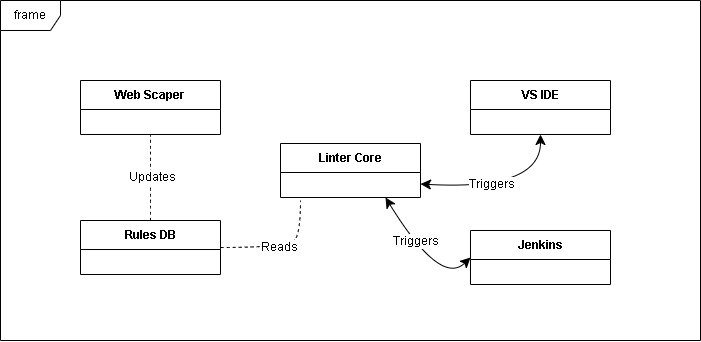
\includegraphics[width=1\linewidth]{Figures/UML.png} % Adjusted width slightly
    \caption{Original Overview of the Implemented Architecture}
    \label{fig:original_architecture} % Changed label for clarity
\end{figure}
The originally envisioned architecture centred around several key components:
\begin{itemize}
    \item A Python backend, likely using Flask, to serve as an API endpoint.
    \item An LLM-based system for automatically generating Regex rules from natural language descriptions of Docker best practices.
    \item A web scraping component (\texttt{BeautifulSoup}) to gather best practices from online sources.
    \item A database (planned as SQLite) to store the generated rules.
    \item A VS Code extension (JavaScript) for IDE integration.
    \item Jenkins integration for CI/CD pipeline checks.
\end{itemize}
This design heavily relied on the successful automation of rule generation via LLMs. (Refer to \refchapfour{} for the detailed initial plan).

\subsection{Final Implemented Architecture}
The architecture implemented by the project deadline is depicted in Figure \ref{fig:final_architecture}.
\begin{figure}[H] % Use [h!] to suggest placing it here if possible
    \centering
    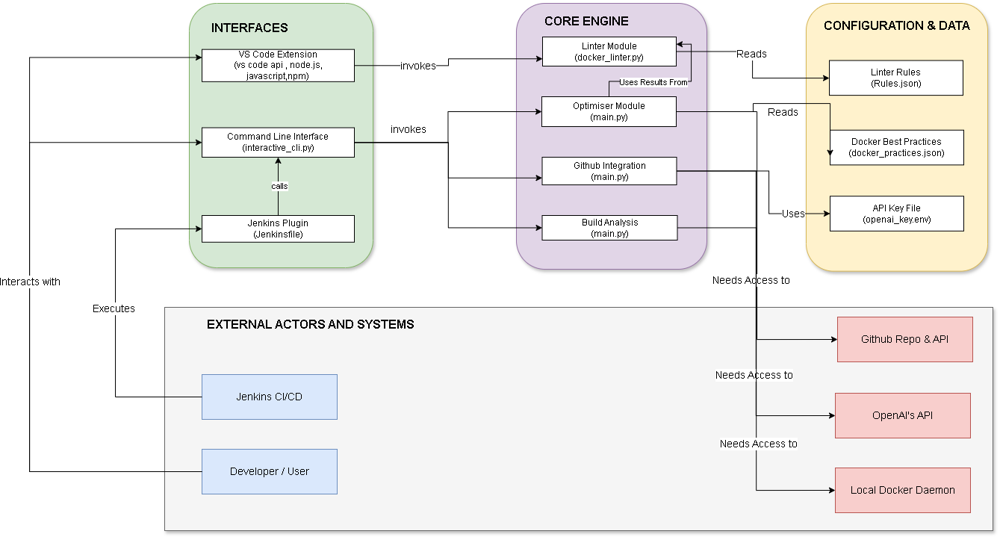
\includegraphics[width=1\linewidth]{Figures/FinalUML.png} % Adjusted width slightly
    \caption{Final Implemented Architecture Overview}
    \label{fig:final_architecture} % Changed label for clarity
\end{figure}

The final system consists of the following core components:
\begin{itemize}
    \item \textbf{Interfaces:} Provides points of interaction for users and external systems.
        \begin{itemize}
            \item \textbf{VS Code Extension (\texttt{VS-Extension}):} Developed using JavaScript/Node.js and the VS Code API to provide real-time linting feedback within the IDE. Invokes the Core Engine.
            \item \textbf{Command Line Interface (\texttt{interactive\_cli.py}):} A Python script allowing direct user interaction and testing. Invokes the Core Engine.
            \item \textbf{Jenkins Plugin (\texttt{Jenkinsfile}):} Enables integration into CI/CD pipelines.
        \end{itemize}

    \item \textbf{Core Engine (Python):} Handles the primary logic of linting, analysis, and integration.
        \begin{itemize}
            \item \textbf{Linter Module (\texttt{dockerfile\_linter.py}):} Performs the fundamental Dockerfile analysis based on the defined rules. Reads from Configuration \& Data.
            \item \textbf{Supporting Modules (\texttt{main.py}):} While shown as separate conceptual blocks in the diagram (Optimiser, GitHub Integration, Build Analysis), these functionalities are implemented within \texttt{main.py}. This includes coordinating analysis,suggesting optimizations (using Linter results), interacting with GitHub APIs, and analysing build information. Reads from and Uses Configuration \& Data. Needs access to External Systems (GitHub API, OpenAI API, Docker Daemon).
        \end{itemize}

    \item \textbf{Configuration \& Data:} Stores the rules, knowledge, and settings used by the Core Engine.
        \begin{itemize}
            \item \textbf{Linter Rules (\texttt{Rules/Rules.json}):} Contains the manually created and validated rule set (Regex patterns, descriptions, suggestions) following the abandonment of LLM-based generation. Read by the Linter Module.
            \item \textbf{Docker Best Practices (\texttt{docker\_practices.json}):} Likely stores structured information gathered by the web scraper (\texttt{webscraper.py}), serving as a knowledge base for AI analysis components or informing manual rule updates. Read by the Core Engine. The scraper itself required ongoing maintenance (\refsubsecreliability{}).
            \item \textbf{API Key File (\texttt{openai\_key.env}):} Stores necessary credentials for accessing external APIs (e.g., OpenAI). Used by the Core Engine.
        \end{itemize}

    \item \textbf{External Actors and Systems (Dependencies):} While not internal components, the system relies on:
        \begin{itemize}
            \item \textbf{Developer/User:} Interacts via VS Code or CLI.
            \item \textbf{Jenkins CI/CD:} Executes the linter via the Jenkins Plugin/CLI.
            \item \textbf{GitHub Repo \& API:} Accessed by the Core Engine for integration features.
            \item \textbf{OpenAI's API:} Accessed by the Core Engine for AI-driven analysis features.
            \item \textbf{Local Docker Daemon:} Accessed by the Core Engine for build analysis or related tasks.
        \end{itemize}
\end{itemize}

\subsection{Comparison and Justification of Changes}

Comparing the initial plan to the final implementation reveals key deviations driven by necessity and practicality:

\begin{itemize}
    \item \textbf{Rule Generation and Storage:} Since using LLMs to automatically generate Regex proved unreliable, we shifted to a fully manual process for creating, checking, and storing rules. We use flat files (Rules) for storage because they are simple and easy to version control. This improved rule quality but slowed development and potentially reduced the number of rules compared to our original automated approach
    \item \textbf{API vs. CLI/IDE Focus:} The planned Flask API was not implemented. Focus shifted to the command-line interfaces  (\texttt{interactive\_cli.py}) and the VS Code extension as the primary methods for users and systems (like Jenkins) to interact with the linter. This provided more direct value for the core developer and CI/CD use cases within the project timeframe, especially given the resources redirected to manual rule creation and scraper maintenance (\refsubsecreliability{}).
    \item \textbf{Use Case Scope:} While the core use cases (CLI linting, IDE feedback, CI/CD checks) were successfully implemented, the scope of "smell detection" was directly tied to the number and quality of manually created rules. The LLM failure (\refsubsecllmregex{}) meant the project couldn't achieve the breadth of automated rule coverage initially hoped for. The "real-time" aspect in the IDE was implemented, but potential latency from external calls (e.g., Python script execution, potential AI analysis calls) needed consideration (\refsubseclatency{}).
    \item \textbf{Risk Realization and Management:} Several planned risks materialized. Web scraper fragility (Risk 10) required ongoing maintenance (\refsubsecreliability{}). CI/CD and IDE integration complexities (Risk 1, Risk 11) were addressed during implementation (\refsubsecintegration{}). An unforeseen major risk emerged regarding the difficulty of translating requirements into reliable rules, especially via LLMs (\refsubsecllmregex{}). The lack of suitable benchmark datasets (\refsubsecbenchmark{}) also presented a challenge during evaluation. Optimizations were applied to the project's own Dockerfile (\refsubsecoptimization{}), potentially mitigating performance risks (Risk 9) for that specific case, though general performance might still be a factor depending on file size and rule complexity.
\end{itemize}

\subsection{(iii) Risk Assessment}
Original Plan: Identified risks including scraper failure, rule conflicts, performance, CI/CD integration issues (Table \ref{tab:ProjRisks}).

Actual Implementation:
\begin{itemize}
    \item The "Web scraper failure" risk (Risk 10) materialized and required ongoing management (Section \ref{subsec:scraper_difficulty}). Mitigation strategies (error handling, monitoring) were crucial.
    \item An unforeseen risk related to the difficulty of translating best practices into rules (especially via automation) emerged and proved significant (Section \ref{subsec:llm_regex_difficulty}).
    \item Risks related to CI/CD or IDE integration (Risk 1, Risk 11) were likely managed during implementation.
\end{itemize}
Deviation: The risk profile shifted, with the rule generation process proving more challenging than initially anticipated.

Justification: Implementation revealed the practical complexities behind some risks (scraper fragility) and uncovered new ones (LLM limitations).

\subsection{(iv) Methodology}
Original Plan: Agile-Scrum methodology.

Actual Implementation: The Agile-Scrum approach appears to have been followed.

Deviation: None explicitly noted, but the methodology's flexibility was likely tested.

Justification: The ability to adapt sprints based on unforeseen challenges like the LLM automation failure (Section \ref{subsec:llm_regex_difficulty}) and scraper maintenance (Section \ref{subsec:scraper_difficulty}) demonstrates the value of the chosen Agile approach. Resources were reallocated from the failing LLM path to manual rule creation.

\subsection{(v) Implementation Schedule}
Original Plan: Detailed Jan-June schedule (Chapter 4, Section 4.4). Jan: Setup, Enhance Prototype; Feb: IDE/DB Integration; Mar: CI/CD, Optimization; Apr: Testing, Reports.

Actual Implementation:
\begin{itemize}
    \item Setup, core linter development, web scraping likely occurred in Jan/Feb.
    \item IDE and CI/CD integration work likely followed.
\end{itemize}
Deviation: The schedule likely experienced delays, particularly in rule set completion and potentially advanced feature testing, due to the time spent on the unsuccessful LLM automation attempt (Section \ref{subsec:llm_regex_difficulty}) and ongoing scraper maintenance (Section \ref{subsec:scraper_difficulty}). Tasks planned for Feb/March might have shifted into March/April. Optimization work (Section \ref{subsec:optimization_difficulty}) also required dedicated time.

Justification: Unforeseen technical hurdles (LLM failure) and the practical demands of maintaining components like the web scraper necessitated schedule adjustments. Prioritization shifted towards ensuring core functionality with manually curated rules.

\subsection{(vi) Evaluation Plan}
Original Plan: Comprehensive plan with quantitative and qualitative metrics, controlled experiments, and real-world testing (Chapter 4, Section 4.5).

Actual Implementation:
\begin{itemize}
    \item The groundwork for evaluation (e.g., linter CLI for testing, potential test cases in `testing/`) was likely laid.
\end{itemize}
Deviation: The scope of the evaluation might have been adjusted based on the final state of the rule set and features. For instance, comparisons against Hadolint/Snyk might focus on a core set of implemented rules due to the manual bottleneck caused by the LLM failure (Section \ref{subsec:llm_regex_difficulty}). Measuring precision/recall might be based on this implemented rule set. Collection of all planned metrics (e.g., latency, developer surveys) might depend on the final implementation status by the end of April.

Justification: The evaluation plan needed to reflect the achievable scope of the project by the deadline, potentially prioritizing validation of the core, manually implemented rules and key integrations over broader comparisons or metrics impacted by the rule generation difficulties.

\subsection{(vii) Prototype}
Original Plan: Included flow charts (Web Scraper, Prioritization), UML diagram, DB schema (Chapter 4, Section 4.6).

Actual Implementation:
\begin{itemize}
    \item The final architecture likely aligns broadly with the UML diagram, showing components like the linter engine, rule storage, scraper, and integrations.
    \item The database schema (`DB/`) might closely follow the prototype, adjusted for manual rule storage.
    \item The web scraper flow likely follows the chart, incorporating the necessary error handling identified as crucial (Section \ref{subsec:scraper_difficulty}).
\end{itemize}
Deviation: The exact implementation details might differ slightly from the initial diagrams based on libraries chosen or refinements made during coding. The rule prioritization logic might have been simplified if the rule set itself was smaller than anticipated post-LLM failure.

Justification: Prototypes serve as a starting point; minor deviations during implementation are normal as technical details are finalized. The core concepts from the prototype likely guided the development.